\chapter{Abstraction}\label{C:abstraction}

% potential examples of abstraction?
% recipies
% programming?
% ???

\begin{displayquote}
 \textit{What is an abstraction?}
\end{displayquote}

A recipie is an abstraction. For example, pumpkin soup:

\begin{enumerate}
\tightlist
\item Boil stock (6 cups), garlic (1 clove), thyme (0.5 tsp) and pumpkin (4 cups) in a pot for 30 mins.
\item Puree the mixture.
\item Simmer for 30 minutes and then add cream (0.5 cups).
\end{enumerate}

This is an abstraction because it captures the essential details: from this recipie, you could make a pumpkin soup.
While it ignores inessential details: the recipe doesn't tell you; where or what to cook in, where to get the
ingredients, how to do the many actions needed to actually puree something, etc...
It also doesn't mandate; the time of day to perform this recipie, what clothes to wear (if any),
which music should be playing, ...

Note that the essential / inessential details will depend on what you want to do with the abstraction.
If we were going to do Y, then it would be important to know ... .

\vspace{5mm}

There exists a mathematical formalism, a  \href{https://en.wikipedia.org/wiki/Homomorphism}{homomorphism},
that allows us to more precisely reason about this transformation from
details to essence. Consider a ground space, $X$, (\textit{the reality of what
needs to be done. all the details.}), and an abstract space $Y$ (\textit{our recipie}).
We are looking for a transformation between $X$ and $Y$ to preserves only the essential
structure in $X$.

% Another way to think about it, a 'structure preserving' map.

\begin{align*}
f(x \diamond_G y) = f(x) \diamond_A f(y)
\end{align*}

Where $f: X\to Y$ is the abstraction. And $\diamond$ is the preserved structure.
Common examples are addition, multiplication. But we might want to preserve the topology of anoperation such as the Bellman operator.

In general, there are three steps to using abstraction to help solve a problem:

\begin{enumerate}
\tightlist
  \item Transform the problem to the 'abstract' domain. $f: X\to Y$
  \item Solve the problem $\mathcal S: Y \to Z$
  \item Lift the solution back to the original domain  $g:Z \to X$
\end{enumerate}

for example.
insert picture of up down etc.

\begin{displayquote}
 \textit{Why do we care?}
\end{displayquote}

The reasons we might care come back to wanting more efficient algorithms.
By throwing away inessential details, there is less to compute.
By throwing away unimportant factors, we have reduced the variance of our
observations and thus allow quicker learning \cite{Allen-Zhu2016a,Johnson2013a}.
% these refs actually show faster convergence now faster learning!?

% History.
%
% - Mathematics, category theory
% - Physics?
% - Comp sci, programming languages

% footnote?
{\color{red}Related. Representation learning.}
% \begin{displayquote}
%   \textit{[Abstraction] is a mapping from one problem representation to a new representation, while preserving some properties} (Littman / Walsh.)
% \end{displayquote}

\section{Abstractions for RL}

% homomorphisms dont segue into this very well...

% types of abstraction we will consider
There are a few different types of abstraction that can be considered for RL:
state abstractions \cite{Anand2019, Littman2006,Haarnoja,Cuccu2018,Zhonga,Vezzani2019,Abel2018,Duan2018,Abel2017,Silver2016a},
action abstractions \cite{Chandak2019,Bester2019,Tennenholtz2019,Nagabandi2019}, state-action abstractions \cite{Dayan1993,Barreto2017}, temporal abstractions \cite{Christodoulou2019, Rafati,Mankowitz2018,Harutyunyan2017,Fruit2017,Riemer2018,Bacon2018,Achiam2018,Pham2019,Konidaris2018,Haarnoja,Sutton1999,Fruit2017a,Bacon2016a,Jinnai2018,Nachum2018}.
These abstractions are often built for two goals; efficient exploration
(\href{https://en.wikipedia.org/wiki/Sample_complexity}{sample complexity})
and / or efficient optimisation (\href{https://en.wikipedia.org/wiki/Computational_complexity_theory}{computational complexity}).

\subsection{Classes of abstraction for RL}

% \begin{displayquote}
% \textit{But how might we contruct $Q^{\pi_{A}^* }$?}
% \end{displayquote}
%
% There are many different forms an abstraction might take, and ???

\begin{displayquote}
\textit{Given an abstraction, how might a learner use it?}
\end{displayquote}

The abstracted $Q$-function and policy might be constructed on spaces $X, Y$,
$Q_A: X \times Y \to \mathbb R$, $\pi_A: X \to \Delta(Y)$. We can now construct
different classes of learners by giving them access to different types of abstraction.

\begin{center}
  \begin{tabular}{ c || c | c | c | c }
    Abstraction & \textbf{X} & \textbf{Y} & \textbf{Value fn} & \textbf{Policy} \\ \hline \hline
    State & $\phi: S \to X$ & $A$ & $Q(\phi(s), a)$ & $\pi(a| \phi(s))$ \\ \hline
    Action & $S$ & $\psi: A \to Y$ & $Q(s, \psi(a))$ & $\pi(\psi^{-1}(y) | s)$\\ \hline
    State and action \footnotemark[5] & $\phi: S \to X$ & $\psi: A \to Y$ & $Q(\phi(s), \psi(a))$ & $\pi(\psi^{-1}(y) | \phi(s))$ \\ \hline
    State-action & \multicolumn{2}{c|}{$\varphi: S\times A \to X\times Y$} & $Q(\varphi(s, a))$ & $\mathop{\text{argmax}}_a Q(\varphi(s, a))$ \\ \hline
    Temporal (goal like) & $S$ & $f: S \to Y$ & $Q(s, f(s))$ &   \\ \hline
    Temporal (option like) & $S$ & $g: \Omega \to Y$ & $Q(s, g(\omega))$ & $\pi(g^{-1}(y) | s)$ \\ \hline
  \end{tabular}
\end{center}

Where $\Omega$ is $A^k$.

\footnotetext[5]{If the $Q$ fn is a linear function of the $\varphi(s, a)$ representation,
then this is known as the successor representation \cite{Dayan1993,Barreto2017}}

\begin{displayquote}
\textit{Which class of abstraction should we use?}
\end{displayquote}

Possibly, the most interesting question is about the difference in performance between
the \textit{State and action abstraction} and the \textit{State-action abstraction}.
Or \textit{goal like} and \textit{option like} temporal abstractions.

The state-action abstraction is the most powerful because it allows the compression of the most symmetries. (want to
prove!)
% The abstraction is able to capture patterns in ??? something about the effects of the actions. Temporal difference models

\subsection{Examples}

\subsubsection{State abstraction}

State abstraction groups together states that are similar. For example,
sprinting 100m is equivalent regardless of which track lane you are in.

If in the forrest, then travel east. If in plains travel south. If at lake, travel east.


\subsubsection{Action abstraction}

Action abstraction groups together actions that are similar. For
example, both action $i$ and action $j$ might yeild the same rewards and change in state,
in which case, we can just relabel them as the same action.

\begin{figure}[h!]
\centering
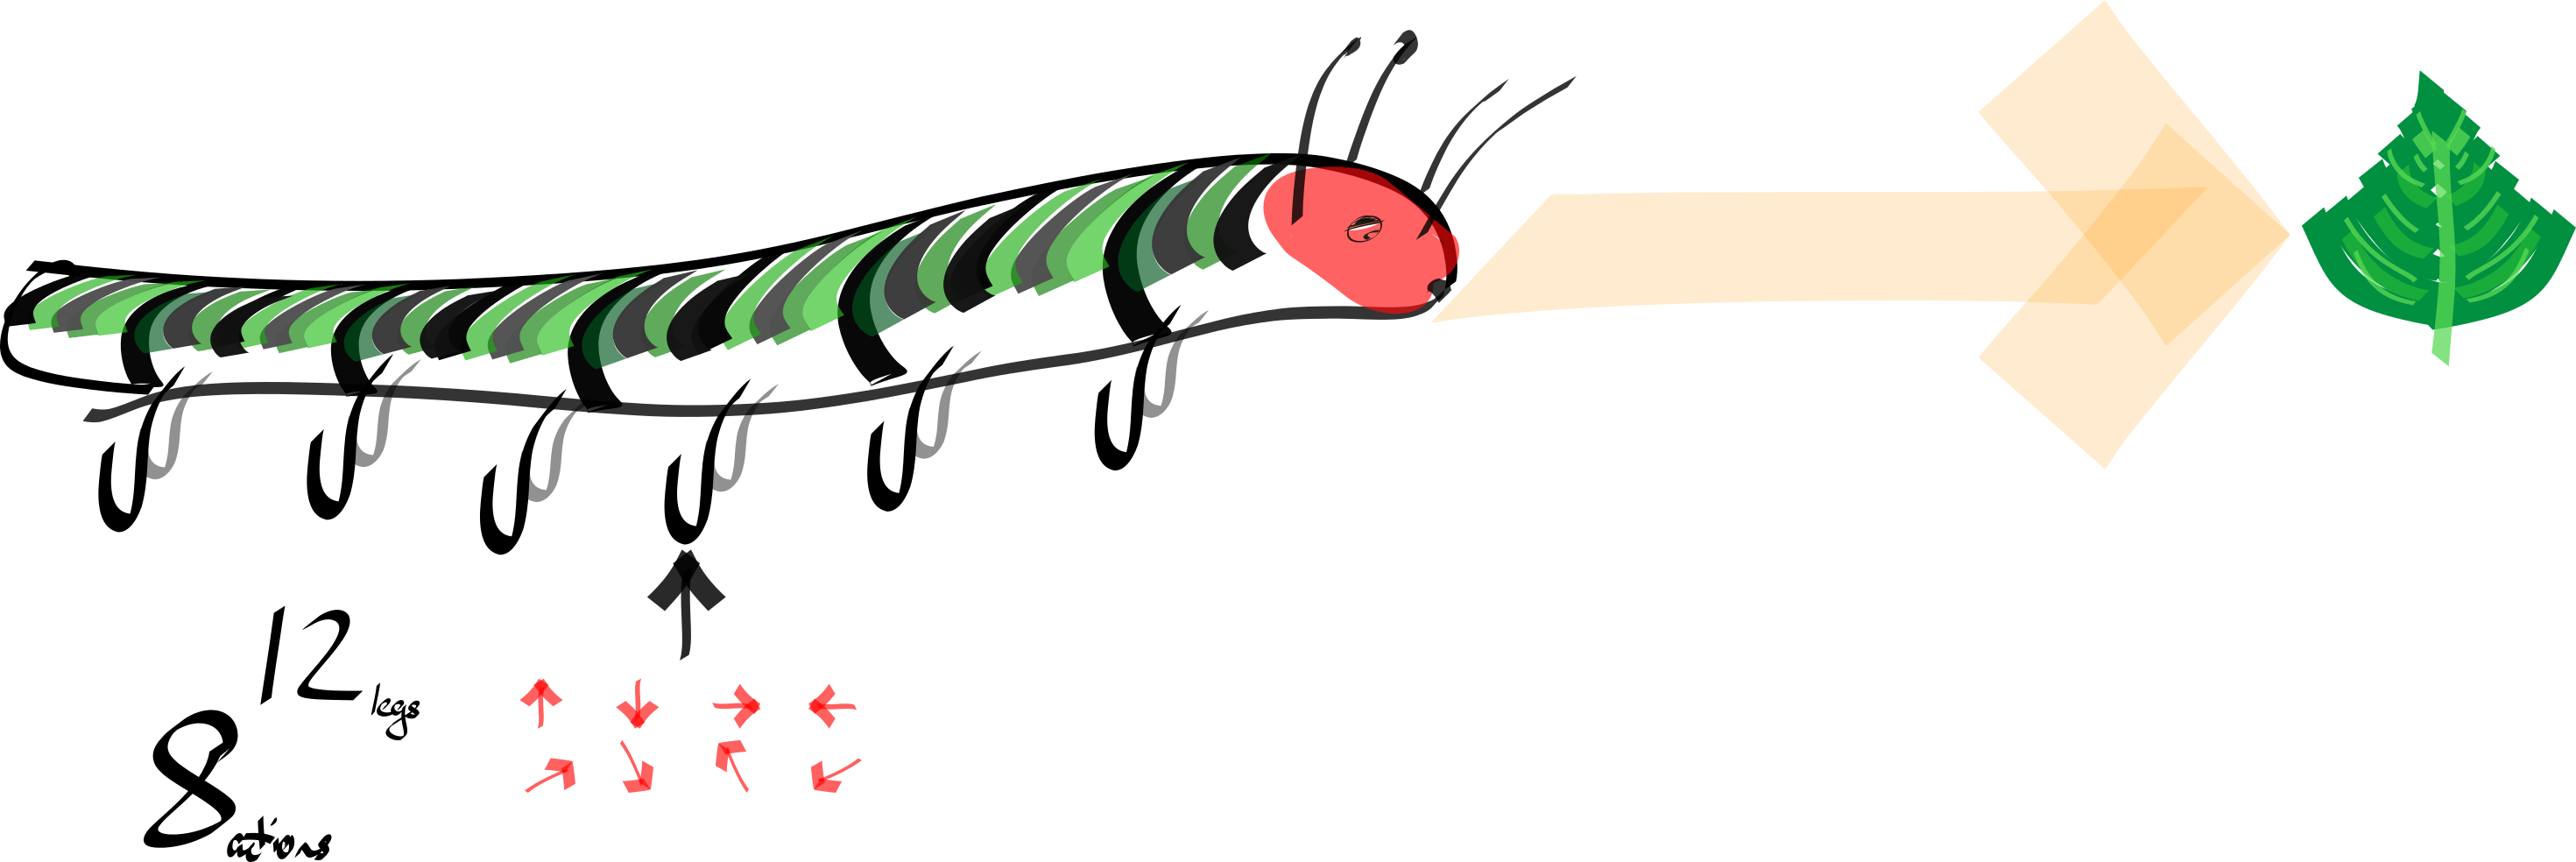
\includegraphics[width=\textwidth,height=0.25\textheight]{../../pictures/drawings/hungry-caterpillar.png}
\caption{Consider a hungry caterpillar. It wants to move towards the leaf. But this is a complicated task! Move your 3rd leg up, your 7th leg down, 11th lag slignly forward, etc...}
\end{figure}


\begin{figure}[h!]
\centering
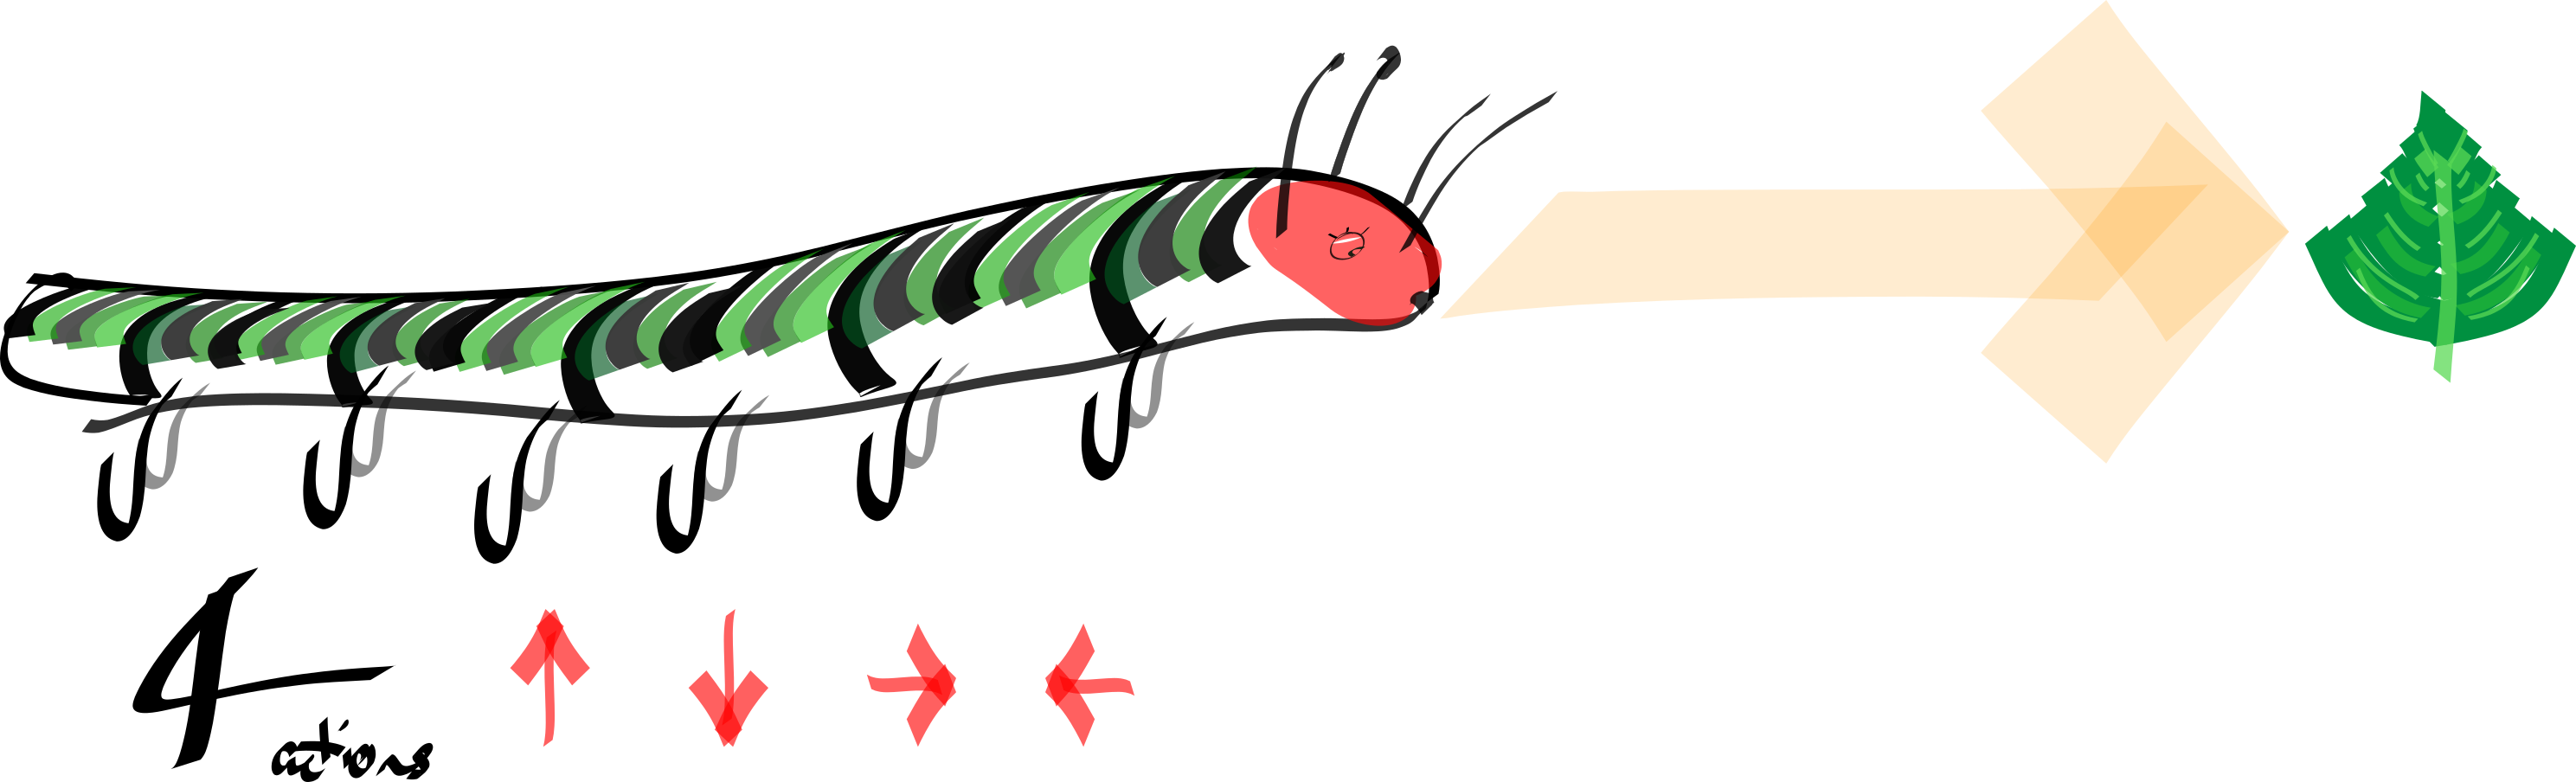
\includegraphics[width=\textwidth,height=0.25\textheight]{../../pictures/drawings/full-caterpillar.png}
\caption{But, what if it could specify actions in another way? Rather than specifying leg movements, it could pick a direction to move, which would specify the movement of multiple legs.}
\end{figure}

\subsubsection{State-action abstraction}

Group together state-actions that achieve similar changes in state and / or changes in future reward.

Imagine you are in a mirror symmetric maze.

\begin{figure}[h!]
\centering
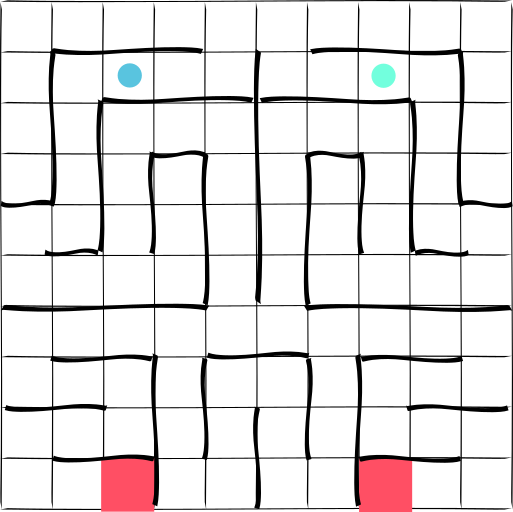
\includegraphics[width=0.8\textwidth,height=0.4\textheight]{../../pictures/drawings/maze.png}
\caption{A symmetric maze, the goal is shown in red.
Consider two different, but the 'same' positions. Shown in blue and green.
In what sense are these two positions the same?}
\end{figure}



This reduces the state-action space by half!
\(\frac{1}{2}\mid S \mid \times \mid A \mid\). Note: just using state
abstraction it is not possible to achieve this reduction. Mirrored
states are not equivalent as the actions are inverted.

While other learners can still solve this problem. They miss out on
efficiency gains by abstracting first.

This intuition leads to our work in section ... (symetric abstractions).

\subsubsection{Temporal abstraction}

???



\subsection{Building an abstraction for RL}

What (structure) do we want to preserve?

% Why is this hard? How hard is it? Existing work? What is the problem?
% How can we find an abstraction? One that actually gives an advantage.
% the cost!!!

% Discovery.
% A complex problem. Versus the cost of discovery plus a simpler problem.
% Need to offset the cost of discovering the abstraction.

% \begin{displayquote}
% \textit{The challenge in the single-task case is overcoming the additional cost of discovering the options; this results in a narrow opportunity for performance improvements, but a well-defined objective. In the skill transfer case, the key challenge is predicting the usefulness of a particular option to future tasks, given limited data.} \cite{Konidaris2019}
% \end{displayquote}


When building an abstraction, you need some notion of how two objects can be similar. (need a ref for this?!)
In RL there are a few possible notions of similarity.

What could be similar? Two states, two actions, two state-actions. Why?
Because they result in the same future rewards? The same future transitions? The same future actions?
Because they can reach the same set of states.

\begin{itemize}
  \tightlist
  \item Characterising the future: One step, k-step, expected, reachable, MC rollout / trajectories, etc etc.
  \item Things we might care about: rewards / fn, actions / fn, states / fn.
  \item All versus just the optimal.
\end{itemize}

If two states have the same value under all possible policies, does this mean
they have the same rewards and transition probabilities?!?

What about $(s_t, a_t, r_t, s_{t+1}, a_{t+1})$s? $(s_t, a_t, r_t, s_{t+1}, a_{t+1})$ and $(s_t', a_t', r_t', s_{t+1}'', a_{t+1}'')$s are similar if?

GVFs

\cite{Littman2006} give 5 classes of state abstraction, and show that ...???
\cite{Abel2017} give 4 classes of approximate states abstraction. They show that ...
Which is best?

Generalise to actions / temporal.

$V(s) - V(s')$ as a similarity measure tells us very little. Because...?
Why doesnt this simple baseline work. Try it out?! Explain.
On a simple MDP, on atari. How to implement? Need to learn $\chi(s, s')$.
It will learn whether two state are similar under many different policys. As we train it...
For every state in our replay buffer, is the return similar to other states?
Just sample a minibatch and compare those states.

Does this allow us to build more general abstractions?

\begin{itemize}
\tightlist
  \item Preserving the ordering of policies. Rather than the absolute value.
  \item Perserving ordering of value. $\phi(s) > \phi(s') \implies Q_{\pi}(s, a) > Q_{\pi}(s', a)$
  \item Preserving the neighborhoods of policies and their values.
  \item ?
\end{itemize}

Want to remove unimportant structure, while keeping the structure that allows us
to exploit the bellman equation (and thus more efficient search).

\subsection{Representation learning}

Examples for representation learning.

Representations that attempt to preserve
\begin{itemize}
\tightlist
  \item the mutual information between ? and ??.
  \item knowledge required to predict the next state
  \item ... geometric bellamere
  \item ?!?
\end{itemize}


\subsubsection{Pairing abstractions with similarity measures}

Different abstraction spaces support different similarity measures.
State similarity based on value fails in rather simple settings.
But works with state-action abstractions!?



\subsection{Analysing abstractions}

\begin{displayquote}
\textit{How might we determine which of these abstractions is better or worse?}
\end{displayquote}

%  but. how can we analyse them?
% tools we can use to analyse an abstraction
Imagine we have a state abstraction, a road is a road: no real difference
between them; gravel, winding, motorway, cliffs-on-either-side...
One of the first things we want to know about the abstraction is:
is it possible for me to act optimally
using this abstraction? If not, what's the damage? In this case, does driving 100kph on every road --
because they are all pretty-much-the-same -- lead to suboptimal results? Probably.
More precisely, we want know to whether the optimal policy can be approximately represented within an abstracted MDP.

% formal
This notion of suboptimality can be formalised as the representation error of the optimal
policy. Given an abstraction, we want to know how well
the abstraction can represent the optimal policy.

\begin{align}
\forall_{s\in S, a\in A} \mid Q^{\pi^* }(s, a) - Q^{\pi_{A}^* }(s, a) \mid \le \epsilon
\end{align}

Where $\pi^{* }$ is the optimal policy, and $\pi_{A}^{* }$ is the lifted optimal
policy found using the abstraction.

While this framework \cite{Littman2006, Abel2017} for analysing
abstraction can tell us that that state abstraction with the preservation of value for all policies
 ...
I does not consider the sample or computational complexity of finding the optimal policy.
Only whether optimal behaviour can be approximately represented.

So the real question we care about has not been answered. Does the abstraction help??

% We need to show that the cost of discovering the abstraction...
% how does this relate to theory on fn approximators?!

\subsection{Discussion}


\begin{itemize}
  \item Abstraction with only preserving optimal actions isnt reliable. We have not preserved the values.
  and therefore, there exist MDPs where the bellman equation is broken, meaning in some cases we cannot learn.
  \item Abstraction that preserves only the value of the optimal policy. So then the value of other policies might be broken.
  How can we still use the bellman eqn to do on-policy learning? We cant? Can only use the bellman optimality eqn / off-policy learning?
  \item When using approximate abstractions, there is some error. This error might accumulate? Needs to be characterised!?
\end{itemize}

% \subsection{Related work}
%
% Existing methods can build abstractions for RL that make solving the problem more computationally efficient.
% These methods work when the model is known, and it can be abstracted...
% When the model is unknown. We might have some belief about likely MDPs. Existing methods do not work on these yet. Too expensive?
% Also. To learn the model with high confidence takes alot of data.
%
% Want symmetry for efficient exploration / sample efficiency.
% Rather than picking actions; randomly, to minimise uncertainty, to ...?
% We want to pick actions to help us identify symmetries in the MDP.
% How does this help us increase the sample efficiency?
%
% Could build this into uncertainty estimates. Where model complexity also factors into the uncertainty estimate (rather than only data).
% Could build this in using ???
%
% If we are using something like neural counts. How does it generalise it density estimates!?
% Want symmetries!!!
